\onehalfspacing
\section{Đề số 30}

\begin{bt} 
    Thực hiện phép tính:
    $$
    \mathrm{A}=\left(1-\frac{1}{2}\right)\left(1-\frac{1}{3}\right)\left(1-\frac{1}{4}\right) ; \quad \mathrm{B}=(0,25)^2 \cdot\left(\frac{1}{3}\right)^{-2}\left(\frac{4}{3}\right)^2 \cdot\left(\frac{1}{4}\right)^{-1}
    $$
\loigiai{
    \begin{enumerate}
        \item $\mathrm{A}=\frac{1}{2} \cdot \frac{2}{3} \cdot \frac{3}{4}=\frac{1}{4}$
        \item $B=\left(\frac{1}{4}\right)^2 \cdot(3)^2 \cdot\left(\frac{4}{3}\right)^2 \cdot 4=\frac{3^2 \cdot 4^2 \cdot 4}{4^2 \cdot 3^2}=4$
    \end{enumerate}
}
\end{bt}

\begin{bt}
    \hfill
	\begin{enumerate}[a.]
        \item Tìm x biết: $|2 x-6|-4 x=12$
        \item Tìm $x$ biết: $\left(\frac{1}{2}+\frac{1}{3}+\ldots+\frac{1}{2015}\right) \cdot x=\frac{2014}{1}+\frac{2013}{2}+\ldots+\frac{2}{2013}+\frac{1}{2014}$
        \item Chứng minh rằng: Nếu $\frac{a}{b}=\frac{c}{d}$ thì $\frac{4 a+5 b}{4 a-5 b}=\frac{4 c+5 d}{4 c-5 d}$
        (Với $a, b, c, d \neq 0 ; 4 a \neq \pm 5 b ; 4 c \neq \pm 5 d$ )
    \end{enumerate}
	\loigiai{
        \begin{enumerate}
            \item Nếu $x \geq 3$ thì: $|2 x-6|-4 \mathrm{x}=12 \Leftrightarrow 2 \mathrm{x}-6-4 \mathrm{x}=12 \Leftrightarrow-2 \mathrm{x}=18 \Leftrightarrow \mathrm{x}=-9$ (KTM)\\[5px]
            Nếu $x<3$ thì: $|2 x-6|-4 \mathrm{x}=12 \Leftrightarrow 6-2 \mathrm{x}-4 \mathrm{x}=12 \Leftrightarrow-6 \mathrm{x}=6 \Leftrightarrow \mathrm{x}=-1$ (TM)\\[5px] 
            Vậy $x=-1$
            \item $\left(\frac{1}{2}+\frac{1}{3}+\ldots+\frac{1}{2015}\right) \cdot x=\frac{2014}{1}+\frac{2013}{2}+\ldots+\frac{2}{2013}+\frac{1}{2014} \\[5px]
            \Leftrightarrow\left(\frac{1}{2}+\frac{1}{3}+\ldots+\frac{1}{2015}\right) x=\frac{2013}{2}+1+\frac{2012}{3}+1 \ldots+\frac{2}{2013}+1+\frac{1}{2014}+1+1 \\[5px]
            \Leftrightarrow\left(\frac{1}{2}+\frac{1}{3}+\ldots+\frac{1}{2015}\right) x=\frac{2015}{2}+\frac{2015}{3}+\ldots+\frac{2015}{2013}+\frac{2015}{2014}+\frac{2015}{2015} \\[5px]
            \Leftrightarrow\left(\frac{1}{2}+\frac{1}{3}+\ldots+\frac{1}{2015}\right) x=2015\left(\frac{1}{2}+\frac{1}{3} \ldots+\frac{1}{2013}+\frac{1}{2014}+\frac{1}{2015}\right) \Leftrightarrow \mathrm{x}=2015 \\[5px]
            \mathrm{KL}: \mathrm{x}=2015$
            \item Với a, b, c, $\mathrm{d} \neq 0,4 \mathrm{a} \neq \pm 5 \mathrm{~b}, 4 \mathrm{c} \neq \pm 5 \mathrm{~d}$, ta có $\frac{a}{b}=\frac{c}{d}
            \Leftrightarrow \frac{a}{c}=\frac{b}{d}$\\[5px]
            Áp dụng TC của dãy tỉ số bằng nhau ta có :\\[5px]
            $\frac{a}{c}=\frac{b}{d}=\frac{4 a}{4 c}=\frac{5 b}{5 d}=\frac{4 a+5 b}{4 c+5 d}=\frac{4 a-5 b}{4 c-5 d} \Leftrightarrow \frac{4 a+5 b}{4 a-5 b}=\frac{4 c+5 d}{4 c-5 d}$
        \end{enumerate}
    } 
\end{bt}

\begin{bt}
    Một vật chuyển động trên các cạnh hình vuông. Trên hai cạnh đầu vật chuyên động với vận tốc $5 \mathrm{~cm} / \mathrm{s}$, trên cạnh thứ ba với vận tốc $4 \mathrm{~cm} / \mathrm{s}$, trên cạnh thứ tư với vận tốc $3 \mathrm{~cm} / \mathrm{s}$. Hỏi độ dài cạnh hình vuông biết rằng tổng thời gian vật chuyển động trên bốn cạnh là 59 giây.
	\loigiai{
        Giả sử thời gian chuyển động trên cạnh thứ nhất, thứ ba, thứ tư lân lượt là x, y, z (giây)\\[5px]
        $\Rightarrow$ thời gian chuyể động trên cạnh thứ hai là x (giây).\\[5px]
        Quãng đường mà vật chuyển động trên các cạnh thứ nhất, thứ ba, thứ tư lân lượt là $5 x, 4 y$, $3 z$.\\[5px]
        Mà độ dài các cạnh của hình vuông bằng nhau nên ta có : $5 x=4 y=3 z$ (1)\\[5px]
        Tổng thời gian vật chuyển động trên bốn cạnh là 59 giây nên có : $x+x+y+z=59$\\[5px]
        Từ (1) $\Rightarrow \frac{x}{4}=\frac{y}{5}, \frac{y}{3}=\frac{z}{4} \Rightarrow \frac{x}{12}=\frac{y}{15}=\frac{z}{20}$\\[5px]
        Áp dụng tính chất của dãy tỉ số bằng nhau ta có : $\frac{x}{12}=\frac{y}{15}=\frac{z}{20}=\frac{2 x+y+z}{24+15+20}=\frac{59}{59}=1$\\[5px]
        $\Rightarrow x=12, y=15, z=20$\\[5px]
        KL : Độ dài cạnh hình vuông là : $5.12=60(\mathrm{~cm})$
    }
\end{bt}

\begin{bt}
    Cho tam giác $A B C$ cân tại $A$. Trên cạnh $B C$ lấy điêm $D$, trên tia đối của tia $C B$ lấy điểm $\mathrm{E}$ sao cho $\mathrm{BD}=\mathrm{CE}$. Các đường thẳng vuông góc với $\mathrm{BC}$ kẻ từ $\mathrm{D}$ và $\mathrm{E}$ cắt $\mathrm{AB}, \mathrm{AC}$ lần lượt ở $M$, $N$.
    \begin{enumerate}[a.]
        \item  Chứng minh rằng: $\mathrm{DM}=\mathrm{EN}$.
        \item $\mathrm{MN}$ cắt $\mathrm{BC}$ tại $\mathrm{I}$.Chứng minh $\mathrm{I}$ là trung điểm của $\mathrm{MN}$.
        \item Chứng minh rằng đường thẳng vuông góc với $\mathrm{MN}$ tại $I$ luôn đi qua một điểm cố định khi $D$ thay đổi trên cạnh $BC$.
    \end{enumerate}
	\loigiai{
        $$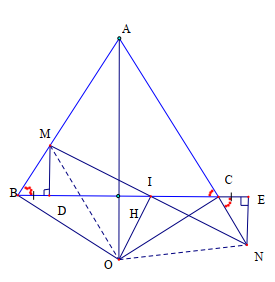
\includegraphics[width=0.45\textwidth]{30-4-lg.png}$$
        \begin{enumerate}
            \item Xét $\triangle B D M=\triangle C E N$ có: $B D=C E(g t)$,\\[5px]
            $D=E=90^{\circ}(\mathrm{MD}, \mathrm{NE} \perp \mathrm{BC}) \\[5px]
            A B C=E C N(=A C B) \\[5px]
            \quad \Rightarrow \triangle \mathrm{BDM}=\triangle \mathrm{CEN}(\text { g.c.g) } \\[5px]
            \Rightarrow \mathrm{DM}=\mathrm{EN}$
            \item Xét $\triangle \mathrm{MDI}$ và $\triangle \mathrm{NEI}$ có: $\quad D=E=90^{\circ}$\\[5px]
            $\mathrm{DM}=\mathrm{EN} \text { ( Theo câu a) }$\\[5px]
            $D M I=E N C$ ( So le trong và $\mathrm{MD} / / \mathrm{NE}$ )\\[5px]
            $\Rightarrow \triangle \mathrm{MDI}=\Delta \mathrm{NEI} \text { ( g.c.g) } \\[5px]
            \Rightarrow \mathrm{IM}=\mathrm{IN}$\\[5px]
            Vậy I là trung điểm của $\mathrm{MN}$.
            \item Gọi $\mathrm{H}$ là chân đường vuông góc kẻ từ $\mathrm{A}$ xuống $\mathrm{BC}, \mathrm{O}$ là giao điểm của $\mathrm{AH}$ với đường thẳng vuông góc với $\mathrm{MN}$ kẻ từ $\mathrm{I} \Rightarrow$ Cần chứng minh $\mathrm{O}$ là điểm cố định.\\[5px]     
            Nối $\mathrm{O}$ với $\mathrm{B}, \mathrm{C}$. Vì đường thẳng $\mathrm{OA}$ cố định nên cần chứng minh $\mathrm{OC}$ cố định hay $\mathrm{OC} \perp$ $\mathrm{AC}$.\\[5px]
            Chứng minh $\triangle \mathrm{OAB}=\triangle \mathrm{OAC}$ (c.c.c) $\Rightarrow O B A=O C A$\\[5px]
            Chứng minh $\triangle \mathrm{OBM}=\triangle \mathrm{OCN}$ ( c.c.c) $\Rightarrow O B A=O C N$\\[5px]
            Từ $1,2 \Rightarrow O C A=O C N$ mà $O C A+O C N=180^{\circ} \Rightarrow O C A=O C N=90^{\circ}$\\[5px]
            $\Rightarrow \mathrm{OC} \perp \mathrm{AC}$.\\[5px]
            $\Rightarrow \mathrm{O}$ là điểm cố định.\\[5px]
            Vậy khi $\mathrm{D}$ di chuyển trên cạnh $\mathrm{BC}$ thì đường thẳng vuông góc với $\mathrm{MN}$ tại $\mathrm{I}$ luôn đi qua một điểm cố định.
        \end{enumerate}
    }
\end{bt}

\begin{bt}
    Cho $f(x)=a x^2+b x+c$ với $a, b, c$ là các số hữu tỉ. Chứng tỏa rằng: $f(-2) \cdot f(3) \leq 0$.

    Biết rằng $13 a+b+2 c=0$
\loigiai{
        $f(-2)=4 a-2 b+c \text { và } f(3)=9 a+3 b+c \Rightarrow f(-2) \cdot f(3)=(4 a-2 b+c)(9 a+3 b+c) \\[5px]
        \text { Nhận thây }(4 a-2 b+c)+(9 a+3 b+c)=13 a+b+2 c=0 \\[5px]
        \Rightarrow(4 a-2 b+c)=-(9 a+3 b+c) \\[5px]
        \text { Vậy } f(-2) \cdot f(3)=-(4 a-2 b+c) \cdot(4 a-2 b+c)=-(4 a-2 b+c)^2 \leq 0$
}
\end{bt}


